\documentclass[class=scrbook, crop=false]{standalone}
\usepackage[subpreambles=true]{standalone}
\ifstandalone
    % WARNING: Proceed with caution!

% -----------------------------------------------------------------------------------
% For package standalone
% -----------------------------------------------------------------------------------
\usepackage{import}

% -----------------------------------------------------------------------------------
% Language and typeset
% -----------------------------------------------------------------------------------
\usepackage[ngerman, english]{babel}

\usepackage{subcaption}
% Umlauts and other special characters (UTF-8)
% \usepackage[utf8]{inputenc}
\usepackage{fontspec}
\setsansfont{Arial}
% \usepackage[T1]{fontenc}  % Enable accented characters and umlauts
% LuaLatex doesn't need fontenc and uses UTF-8
% \usepackage{lmodern}  % Font face


% --------------------------------------------------------------------------------
% Page formatting
% --------------------------------------------------------------------------------
% Change the header/footer for chapter beginnings and normal pages
\usepackage[automark,headsepline]{scrlayer-scrpage}

% The package provides an easy and flexible user interface to customize the page
% layout, implementing auto-centering and auto-balancing mechanisms
% WARNING: WHEN CHANGING BCOR (Binding correction), the cover needs reworking!...
\newcommand{\theBCOR}{15mm}  % Define binding correction
\usepackage[
    bindingoffset=\theBCOR,
    % showframe, % Show boxes which indicate margins and paddings
    bottom = 3.5cm, % Margins
      left = 2.5cm,
     right = 2.5cm
] {geometry}

% The package 'float' provides a container for document objects which can not be
% broken over pages, such as tables and figures
% Needed for table and figure indexes  
\usepackage{float}

% support for landscape layout
\usepackage{lscape}

% support of \tablenotes command to add notes under table
\usepackage{threeparttable}

% To allow drawing more professional tables
\usepackage{booktabs}

% --------------------------------------------------------------------------------
% Contents
% --------------------------------------------------------------------------------
% Vector graphics (for Cover page)
\usepackage{tikz} 

% Allows additional parameters when including images
\usepackage{graphicx}

% Roman font family for all headings
\addtokomafont{disposition}{\rmfamily}

% Set the line spacing to 1.5
\usepackage[onehalfspacing]{setspace}

% Improves overall text spacing
% http://www.khirevich.com/latex/microtype/
\usepackage[stretch=10]{microtype}

% Math symbols like mu outside the math environment
\usepackage{textcomp}

% A comprehensive (SI) units package∗
% For defining SI units
\usepackage[
    range-units=single,         % Formatting ranges with single unit indication: 1 - 2 m
    range-phrase=-,             % Phrase for range: 1 - 2 m vs 1 to 2 m
    separate-uncertainty=true,  % sets +- between value and uncertainty 
    multi-part-units=repeat     % In expressions with multiple values (multi part numbers) 
                                % the unit is printed each time: 1 mm x 1 mm
] {siunitx}
% https://tex.stackexchange.com/questions/124488/multi-part-numbers-and-units-in-siunitx

% Allows Sourcecodes with highlighting 
\usepackage{listings}

% This package provides user control over the layout of the three basic list
% environments: enumerate, itemize and description
\usepackage{enumitem}
\setlist{nosep} % Remove the vertical space between \item elements in all lists

% ToDo Notes
% \setlength{\marginparwidth}{2cm}
\usepackage{todonotes}
\setuptodonotes{inline, inlinepar}
\reversemarginpar  % Put ToDo notes on the binding's side
% \usepackage{soul} % Colorful ToDo notes

% Check out colors here http://latexcolor.com/
\usepackage{xcolor}

\usepackage{amsmath}    % alignment of equations

% --------------------------------------------------------------------------------
% Other elements
% --------------------------------------------------------------------------------
% Blindtext: Organic looking text dummy
\usepackage{blindtext}

% Hyperlinks within the document (PDF)
% "hidelinks" hides visual highlighting of links
\usepackage[hidelinks]{hyperref}

% Package for Glossary and Index (Acronyms are listed in a separate list) 
\usepackage[acronym, nogroupskip]{glossaries}[=v4.49] % groupskip: alphabetic grouping of entries

\usepackage{xltabular}   % <------- FOR glossaries

% Integration and management of bibliographies
\usepackage{csquotes}   % backend=biber in biblatex needs this package
\usepackage[
    style=ieee,   % style of the bibliography, entries are sorted in alphabetic order. "ieee" is another common style.
    backend=biber,      % based on package 'biber' 
    bibencoding=ascii   % ASCII Text encoding; may use "utf8" instead
] {biblatex}

% --------------------------------------------------------------------------------
%                               PATHS & FILES
% --------------------------------------------------------------------------------
% Fix paths for standalone compiling
\ifstandalone
    \def \home {..}
\else
    \def \home {.}
\fi

% Package: scrlayer-scrpage
% \def \stylePath {\home/settings+/style/page}
\input{\home/settings+/style/page}  % Load page style

% Package: graphicx
\graphicspath{{\home/images/}}  % Set path to images

% Package: listings
\input{\home/settings+/style/code.tex}  % Set path to style file
\lstset{inputpath={\home/code/}} % Default path to code listings

% Package: glossaries
\input{\home/settings+/style/symbols}  % Set path to symbols list style file
\input{\home/settings+/style/acronyms}  % Set path to acronym list style file
% -------------------------------------------------------------------------------
%               Listing of all Glossary and Acronym Entries 
%                           use as shown below
% -------------------------------------------------------------------------------

% ==== EXEMPLARY ENTRY FOR SYMBOLS LIST =========================================

% ==== EXEMPLARY ENTRY FOR ACRONYMS LIST ========================================
% \newacronym{#label}{#acronym}{#long_form}

% define new command for custom arconym entry with only two arguments
% fabricates an easier way to use \newacronym 
\newcommand{\acroX}[2]{\newacronym{#1}{#1}{#2}}
% \acroX{label and arconym}{long name}
% \acroX{CD}               {Compact Disk}

\newcommand{\acroY}[3]{\newacronym{#1}{#2}{#3}}
% \arcoY{label}{acronym}{long name}
% \acroY{CD}   {cd}     {Compact Disk}
 
\newacronym{AEP}{AEP}{Imbalance price}
\newacronym{aFRR}{aFRR}{Automatic Frequency Restoration Reserve}


\newacronym{reBAP}{reBAP}{Uniform imbalance price}
\newacronym{TSO}{TSO}{Transmission System Operator}
\newacronym{FCR}{FCR}{Frequency Containment Reserve}
\newacronym{mFRR}{mFRR}{Manual Frequency Restoration Reserve}
\newacronym{BRP}{BRP}{Balancing Responsible Party}
\newacronym{SB}{SB}{System Balance}
\newacronym{VRE}{VRE}{variable renewable energy}
\newacronym{ID1}{ID1}{intraday index ID1}
\newacronym{MAE}{MAE}{mean average error}
\newacronym{RMSE}{RMSE}{root mean squared error}
\newacronym{MSE}{MSE}{mean squared error}
\newacronym{CRPS}{CRPS}{continuous ranked probabililty score}
\newacronym{GCC}{GCC}{Grid Control Cooperation}
\newacronym{IC}{IC}{Continuous intraday}
\newacronym{VWAP}{VWAP}{volume-weighted average price}
\newacronym{VID}{VID}{traded volume within the intraday market}
\newacronym{ID AEP}{ID AEP}{Intraday Average Energy Price}
\newacronym{FRR}{FRR}{Frequency Restoration Reserve}
\newacronym{TFT}{TFT}{Temporal Fusion Transformer}
\newacronym{DLM}{DLM}{Dynamic Linear Model}
\newacronym{GB}{GB}{Gradient Boosting}
\newacronym{RF}{RF}{Random Forest}
\newacronym{ARIMAX}{ARIMAX}{Autoregressive Integrated Moving Average with eXogenous variables}
\newacronym{xLSTM}{xLSTM}{Extended Long Short-Term Memory}
\newacronym{DWD}{DWD}{Deutscher Wetterdienst}
\newacronym{ENTSO-E}{ENTSO-E}{European Network of Transmission System Operators for Electricity}
\newacronym{IDA1}{IDA1}{Intraday auction 1}
\newacronym{MOSMIX}{MOSMIX}{Model Output Statistics-MIX}
\newacronym{mLSTM}{mLSTM}{memory-optimized LSTM}
\newacronym{sLSTM}{sLSTM}{speed-optimized LSTM}

% ==== EXEMPLARY ENTRY FOR MAIN GLOSSARY ========================================

    % \newglossaryentry{policy}{name={Policy},description={Im geschäftlichen Bereich bezeichnet Policy eine interne Leit- bzw. Richtlinie, die formal durch das Unternehmen dokumentiert und über ihr Management verantwortet wird}}
    % \newglossaryentry{pcie}{name={PCI Express},description={PCI Express („Peripheral Component Interconnect Express“, abgekürzt PCIe oder PCI-E) ist ein Standard zur Verbindung von Peripheriegeräten mit dem Chipsatz eines Hauptprozessors. PCIe ist der Nachfolger von PCI, PCI-X und AGP und bietet im Vergleich zu seinen Vorgängern eine höhere Datenübertragungsrate pro Pin.}}
    % \newglossaryentry{realnumber}
  % Load glossary, symbol and acronyms list

% Package: biblatex
\addbibresource{\home/references/references.bib}  % Set path to bib resources

% Custom variables
\input{\home/settings+/variables}
% --------------------------------------------------------------------------------
%                                   OPTIONAL
% --------------------------------------------------------------------------------


% Simple arithmetic for LaTeX commands
% \usepackage{calc}

% Document Elements
% -------------------

% Index
% \usepackage{imakeidx}

% compact Lists
%\usepackage{paralist}

% visual improvements for citations
% \usepackage{epigraph}

% Create pseudo code
% https://www.overleaf.com/learn/latex/Algorithms
% \usepackage{algorithm}
% \usepackage{algorithmic}
%\usepackage[noend]{algpseudocode}

% Formatting
% -------------------
% Tweaks for scrbook, redefines commands of other packages
% \usepackage{scrhack}

% Intelligent space separator (nice for superscript?)
% \usepackage{xspace}

% Allows breaks within tables
%\usepackage{tabularx}

% Allows for page breaks in tables
% \usepackage{longtable}

% allows modifying of captions
% \usepackage{caption}

% Multiline comments
%\usepackage{verbatim}

% % Custom colors
% \definecolor{dartmouthgreen}{rgb}{0.05, 0.5, 0.06}

% IF you want to define unicode characters
% \DeclareUnicodeCharacter{0229}{\c{e}}
% \DeclareUnicodeCharacter{0306}{\u{Z}}


% Document elements
% ------------------------------------

% Table package
% \usepackage{booktabs}

% Pie diagram
% \usepackage{datapie}

% Side by Side images
% \usepackage{subcaption}

% For landscape tables
%\usepackage{pdflscape}
%\usepackage{afterpage}

% Graphics can be flow around by text
%\usepackage{wrapfig}

\fi

% ----------------------------------------------------------------------------
%                               Theoretical Background
% ----------------------------------------------------------------------------
\begin{document}

\ifstandalone
    \selectlanguage{ngerman}  % Toggle ON/OFF

    % Language-specific settings that change automatically
    \input{settings+/language}
\fi

\chapter{Theoretical Background}
\label{Chapter::Theoretical_Background} % Outline text
This chapter provides background knowledge to understand the concepts in the thesis.

% Background topics that are necessary to understand your thesis
\section{German electricity market}
\label{Section::German_Electricity_Market}

In the german electricity market every market participant is a BRP. Each BRP has to balance their portfolio so that their generation matches their consumption. Both of these values are partially unknown and can deviate. 
Energy generation can have many sources, for VRE the produced energy heavily depends on the current weather.
To estimate the energy generated by VRE information about weather situations can be used to get an approximation. 

As well as the generation, consumption of energy also is not fixed. The consumption of energy varies with social constructs, such as the work week, holidays or school holidays. 
BRPs have access to past data to make an informed decision and submit a schedule when they will insert how much energy into the system.
This schedule is submitted to the TSOs.

The physically delivered volumes might differ from these schedules, for example due to a bad weather forecast. In this case the BRP has an imbalanced portfolio.
The deviation in all portfolios of all BRPs in a balancing area are summed up and the result is the system balance (SB) for that balancing area. Summed up across all balancing areas this is the grid control network system balance.

To keep the grid at 50hz frequency, TSOs have to dispatch balancing energy according to the system balance. This energy can be positive, if the grid is short of energy, or negative, if the grid has a surplus of energy. 

If the system is in need of energy reserve generators that run below full capacity can be activated to increase their production. Another way of introducing positive balancing energy into the grid is turning off variable loads to decrease energy consumption.

If the system has a surplus of energy, negative balancing energy has to be dispatched. This can be done either by throttleing capacity generators which are running above minimum capacity. Negative balancing energy can also be inserted into the grid by turning on variable loads, leading to an increased energy consumption.

Now every BRPs portfolio is balanced using this balancing energy. For this the imbalance price is calculated. How this price is calculated will be explained in the next chapter.
Each BRP whose portfolio led to increasing the system balance, for example having provided not enough energy whilst the system is also short of energy, has to pay the imbalance price for the volume of their imbalance. 
On the other hand, BRPs which helped stabilize the system with their portfolio, for example providing more energy than consumed while the system is short of energy, are remunerated for their imbalance. 

Next, the different auctions and their schedule will be explained. An overview can be found in \ref{fig::energy_auctions}. 

\begin{figure}[ht]
            \centering
            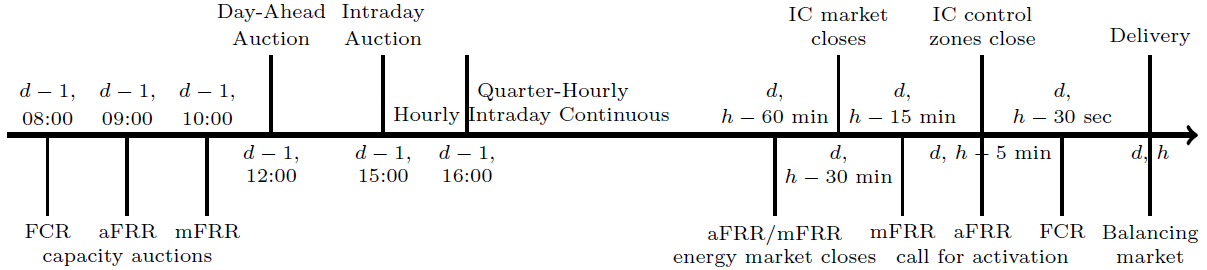
\includegraphics[width=\textwidth]{theory/energy_auctions.png}
            \caption[Timeschedule for energy market auctions]{Timeschedule for energy market auctions \cite{narajewskiProbabilisticForecastingGerman2022}.}
            \label{fig::energy_auctions}
 \end{figure}
 
 On the far right of the figure the time of delivery is shown, denoted by $d$, $h$ of the delivery. The auctions for this timestamp start the day before. From $8:00$ to $10:00$ on the previous day reserve capacity auctions take place. These auctions decide how positive and negative balancing energy is introduced into the system when balancing the grid. During this auctions will not play any role, as data for these auctions was not available at the time of the experiments. 
The first auction takes place at $12:00$ one day before delivey and is called the day ahead (DA) auction. At $15:00$ the next auction, the intraday auction (IA) takes place. After that, at $16:00$ intraday continuous trading (IC) starts. Whilst the auctions are a single auction event, during the intraday continuous (IC) trading window energy can be traded at any time. The IC has different closing times. Up until $30$ minutes before delivery energy can be traded across all control zones. Trades on IC that happen within a single control zone can be done up until $5$ minutes before delivery.

\section{Imbalance price}
\label{Section::Imbalance_Price}
The calculation of the imbalance price is split up into three modules, which are calculated seperately and subsequently aggregated.

\subsection{Module 1: Basis component}
The first module is called the basis component. 
This module represents the cost of providing the balancing energy.

With information provided by PICASSO the volume-weighted average price for the automatic frequency restoration reserve $VWAP_{aFRR}$ can be calculated. This is calculated for both positive and negative activations, resulting in $VWAP_{aFRR, GCC, pos, qh}$ and $VWAP_{aFRR,  GCC, neg, qh}$ for each quarter hour $qh$ and the GCC balance.
The same calculations are done for mFRR activations using data from MARI, resulting int $VWAP_{mFRR, GCC, pos, qh}$ and $VWAP_{mFRR, GCC, neg, qh}$. 
These valuese are used in the formulas \ref{fig::aep1_pos} and \ref{fig::aep1_neg} to calculate the values $AEP1_{pos}$ and $AEP1_{neg}$. 
If neither aFRR or mFRR were activated during the associated quarter hour this $AEP1$ takes the value of avoided activation. This value is equal to the mean of the cheapest aFRR bid prices for the quarter hour.
If only one of the reserves was activated $AEP1$ takes the value of the $VWAP$ of that reserve. 
If both reserves were activated, the $AEP1$ is equal to the volume-weighted average of both $VWAPs$. The volume is denoted by the satisfied demand $SD$.

\begin{figure}[ht]
            \centering
            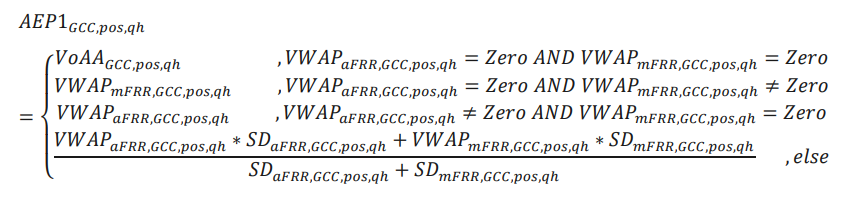
\includegraphics[width=\textwidth]{theory/aep1_pos.png}
            \caption[Positive AEP 1 component formula]{Positive AEP 1 component formula \cite{NetztransparenzReBAP}.}
            \label{fig::aep1_pos}
 \end{figure}
 
 

 \begin{figure}[ht]
            \centering
            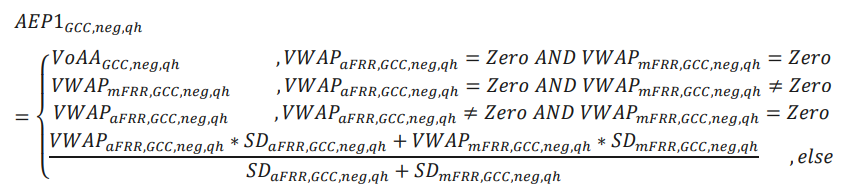
\includegraphics[width=\textwidth]{theory/aep1_neg.png}
             \caption[Positive AEP 1 component formula]{Positive AEP 1 component formula \cite{NetztransparenzReBAP}.}
            \label{fig::aep1_neg}
 \end{figure}

With both $AEP1s$, the value of the basis component can be calculated. If the system balance is positive, this module takes the value of $AEP1_{GCC, pos, qh}$. If the system balance is negative, this module takes the value of $AEP1_{GCC, neg, qh}$. If the system balance is equal to 0, this module's value is 0.

\subsection{Module 2: Incentivising component}

The goal behind module 2 is to increase the reBAP, so that it is more costly to use imbalance energy than buying the need energy on the intraday market. This should incentivise all BRPs to keep their portfolio balanced. 
The formula for its calculation is displayed in figure \ref{fig::aep2}.and will be explained in the next paragraphs.

For each settlement period $V_{ID}$ denotes the volume of total trades that were closed on the intraday market for this quarter. If this volume is below $500$MW, this component finds no application and takes the value of 0. If value was greater than $500$MW this module is calculated using the Intraday Price Index (ID AEP) and a minimum distance $\Delta P$. 
The ID AEP is calculated for each quarter hour by averaging over the trades closest to the delivery time. For this calculation only a volume of 500 MW, so 125 MW/h for a quarter hour is considered.  
The volume-weighted average price is formed from the transactions filtered this way. 
In the case that the GCC balance is equal to 0, this module takes the value of ID AEP.  In the case of a positive GCC balance, a minimum distance $\Delta P$ is added onto the ID AEP, in case of a negative GCC balance this $\Delta P$ is substracted from the ID AEP. Between ID AEP and module 2 a minimum distance of $25\%$, but at least 10€ is established, assuming the absolute value of the GCC balance is equal to or greater than $500$ MW. This distance $\Delta P$ linearly ramps up from $0$MW to $500$MW. The formula for $\Delta P$ can be found in figure \ref{fig::delta_p} and a graph for its values with a fixed ID AEP of $100€/MWh$ is displayed in figure \ref{fig::delta_p_graph}.

 \begin{figure}[ht]
            \centering
            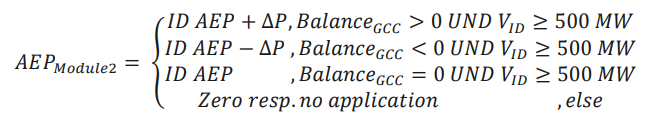
\includegraphics[width=\textwidth]{theory/aep_2.png}
             \caption[Formula for $AEP_{Module 2}$]{Formula for $AEP_{Module 2}$ \cite{NetztransparenzReBAP}.}
            \label{fig::aep2}
 \end{figure}

 \begin{figure}[ht]
            \centering
            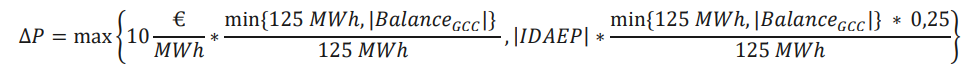
\includegraphics[width=\textwidth]{theory/delta_p.png}
             \caption[Formula for$ \Delta P$]{Formula for $\Delta P$ \cite{NetztransparenzReBAP}.}
            \label{fig::delta_p}
 \end{figure}
 
 \begin{figure}[ht]
            \centering
            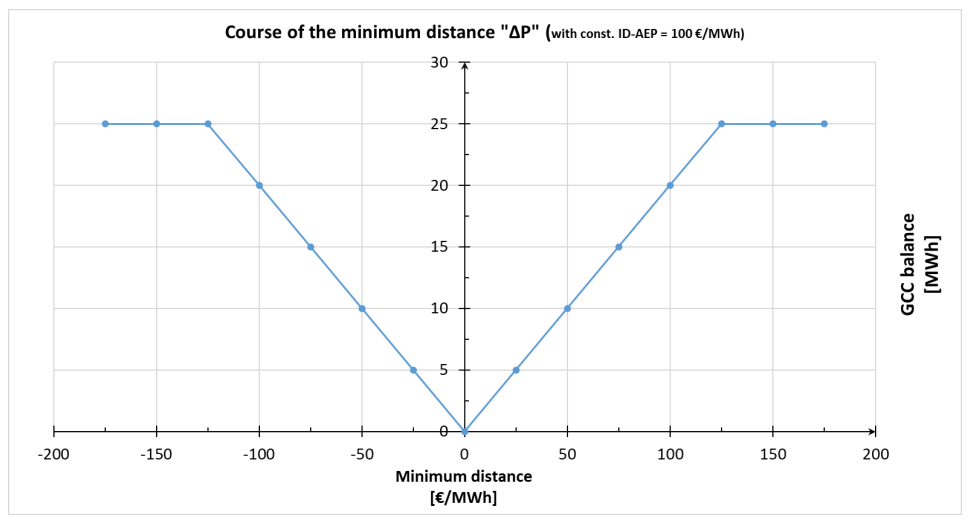
\includegraphics[width=\textwidth]{theory/delta_p_graph.png}
             \caption[Graph for $\Delta P$ with a fixed ID AEP for $100€/MWh$ \cite{NetztransparenzReBAP}]{Graph for $\Delta P$ with a fixed ID AEP for $100€/MWh$ \cite{NetztransparenzReBAP}.}
            \label{fig::delta_p_graph}
 \end{figure}

\subsection{Module 3: Scarcity component}

If the GCC balance exceeds $80\%$ of the frequency restoration reserve (FRR) for a settlement period, the scarcity component is applied. This component rarely is the price setting module of the reBAP (<1\%). The formula for this module will not be discussed here. Figure \ref{fig::aep_3} shows a graph of how this module's value changes relatively to the GCC balance.


 \begin{figure}[ht]
            \centering
            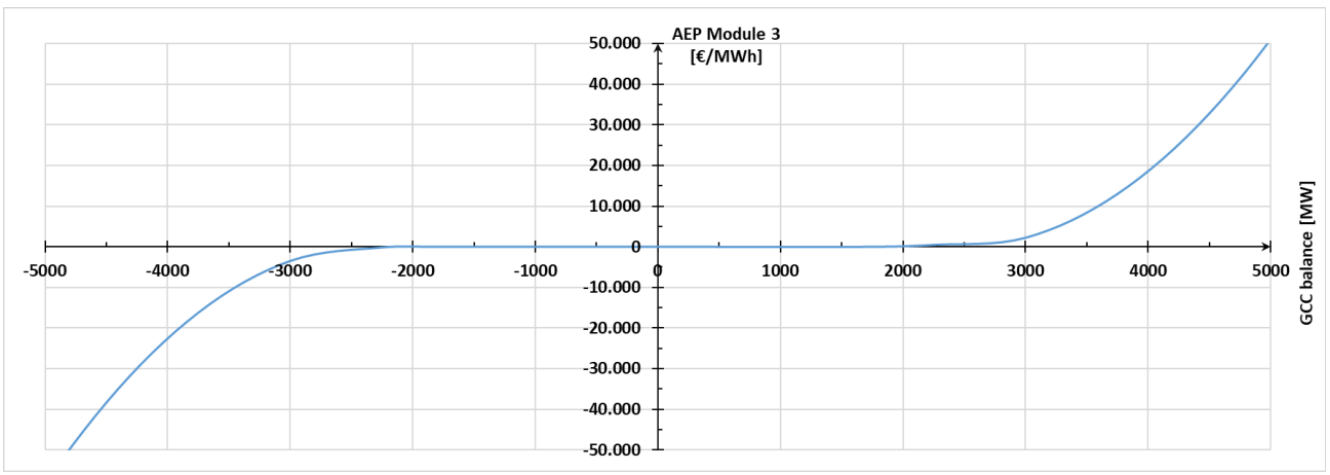
\includegraphics[width=\textwidth]{theory/aep_3.png}
             \caption[Graph how the price of module 3 correlates with GCC balance$ \cite{NetztransparenzReBAP}]{Graph how the price of module 3 correlates with GCC balance \cite{NetztransparenzReBAP}.}
            \label{fig::aep_3}
 \end{figure}


Depeding on the sign of the GCC balance, either the minimum or the maximum of the three modules introduced in the previous paragraphs is used. The formula for this is displayed in figure \ref{fig::rebap_neg}. If the GCC balance is positive, the module with the highest value is used. If the balance is negative the cheapest module is used to determine the reBAP.

For the whole year 2024 the reBAP was equal to the basis component $82.76\%$, equal to the incentivising component $17.23\%$ and equal to the scarcity component $0.00\%$ of the time, with the scarcity component only being the price setting module once throughout 2024. This data is displayed in figure \ref{fig::aep_modules}.

 \begin{figure}[ht]
            \centering
            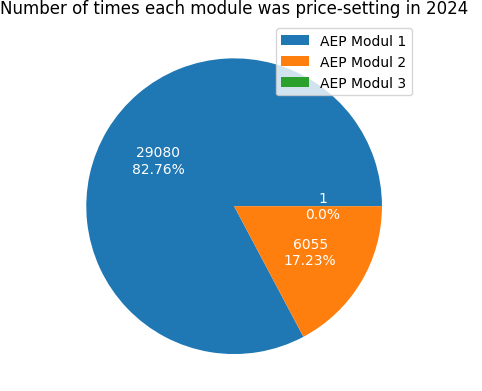
\includegraphics[width=.5\textwidth]{theory/aep_modules.png}
             \caption[How often each module was price-setting in 2024?]{How often each module was price-setting in 2024?}
            \label{fig::aep_modules}
 \end{figure}



% You can use this to add content for standalone documents if you like
% In this case we would like to show the references.
\ifstandalone
    % Bibliography
    \printbibliography[heading=bibintoc]                         \cleardoublepage

% ----------------------------------------------------------------------------
% Appendix and Glossary
% ----------------------------------------------------------------------------
%     \pagenumbering{Alph} % A, B, C..

% %     % Appendix
%     \documentclass[class=scrbook, crop=false]{standalone}
\usepackage[subpreambles=true]{standalone}
\ifstandalone
    % WARNING: Proceed with caution!

% -----------------------------------------------------------------------------------
% For package standalone
% -----------------------------------------------------------------------------------
\usepackage{import}

% -----------------------------------------------------------------------------------
% Language and typeset
% -----------------------------------------------------------------------------------
\usepackage[ngerman, english]{babel}

\usepackage{subcaption}
% Umlauts and other special characters (UTF-8)
% \usepackage[utf8]{inputenc}
\usepackage{fontspec}
\setsansfont{Arial}
% \usepackage[T1]{fontenc}  % Enable accented characters and umlauts
% LuaLatex doesn't need fontenc and uses UTF-8
% \usepackage{lmodern}  % Font face


% --------------------------------------------------------------------------------
% Page formatting
% --------------------------------------------------------------------------------
% Change the header/footer for chapter beginnings and normal pages
\usepackage[automark,headsepline]{scrlayer-scrpage}

% The package provides an easy and flexible user interface to customize the page
% layout, implementing auto-centering and auto-balancing mechanisms
% WARNING: WHEN CHANGING BCOR (Binding correction), the cover needs reworking!...
\newcommand{\theBCOR}{15mm}  % Define binding correction
\usepackage[
    bindingoffset=\theBCOR,
    % showframe, % Show boxes which indicate margins and paddings
    bottom = 3.5cm, % Margins
      left = 2.5cm,
     right = 2.5cm
] {geometry}

% The package 'float' provides a container for document objects which can not be
% broken over pages, such as tables and figures
% Needed for table and figure indexes  
\usepackage{float}

% support for landscape layout
\usepackage{lscape}

% support of \tablenotes command to add notes under table
\usepackage{threeparttable}

% To allow drawing more professional tables
\usepackage{booktabs}

% --------------------------------------------------------------------------------
% Contents
% --------------------------------------------------------------------------------
% Vector graphics (for Cover page)
\usepackage{tikz} 

% Allows additional parameters when including images
\usepackage{graphicx}

% Roman font family for all headings
\addtokomafont{disposition}{\rmfamily}

% Set the line spacing to 1.5
\usepackage[onehalfspacing]{setspace}

% Improves overall text spacing
% http://www.khirevich.com/latex/microtype/
\usepackage[stretch=10]{microtype}

% Math symbols like mu outside the math environment
\usepackage{textcomp}

% A comprehensive (SI) units package∗
% For defining SI units
\usepackage[
    range-units=single,         % Formatting ranges with single unit indication: 1 - 2 m
    range-phrase=-,             % Phrase for range: 1 - 2 m vs 1 to 2 m
    separate-uncertainty=true,  % sets +- between value and uncertainty 
    multi-part-units=repeat     % In expressions with multiple values (multi part numbers) 
                                % the unit is printed each time: 1 mm x 1 mm
] {siunitx}
% https://tex.stackexchange.com/questions/124488/multi-part-numbers-and-units-in-siunitx

% Allows Sourcecodes with highlighting 
\usepackage{listings}

% This package provides user control over the layout of the three basic list
% environments: enumerate, itemize and description
\usepackage{enumitem}
\setlist{nosep} % Remove the vertical space between \item elements in all lists

% ToDo Notes
% \setlength{\marginparwidth}{2cm}
\usepackage{todonotes}
\setuptodonotes{inline, inlinepar}
\reversemarginpar  % Put ToDo notes on the binding's side
% \usepackage{soul} % Colorful ToDo notes

% Check out colors here http://latexcolor.com/
\usepackage{xcolor}

\usepackage{amsmath}    % alignment of equations

% --------------------------------------------------------------------------------
% Other elements
% --------------------------------------------------------------------------------
% Blindtext: Organic looking text dummy
\usepackage{blindtext}

% Hyperlinks within the document (PDF)
% "hidelinks" hides visual highlighting of links
\usepackage[hidelinks]{hyperref}

% Package for Glossary and Index (Acronyms are listed in a separate list) 
\usepackage[acronym, nogroupskip]{glossaries}[=v4.49] % groupskip: alphabetic grouping of entries

\usepackage{xltabular}   % <------- FOR glossaries

% Integration and management of bibliographies
\usepackage{csquotes}   % backend=biber in biblatex needs this package
\usepackage[
    style=ieee,   % style of the bibliography, entries are sorted in alphabetic order. "ieee" is another common style.
    backend=biber,      % based on package 'biber' 
    bibencoding=ascii   % ASCII Text encoding; may use "utf8" instead
] {biblatex}

% --------------------------------------------------------------------------------
%                               PATHS & FILES
% --------------------------------------------------------------------------------
% Fix paths for standalone compiling
\ifstandalone
    \def \home {..}
\else
    \def \home {.}
\fi

% Package: scrlayer-scrpage
% \def \stylePath {\home/settings+/style/page}
\input{\home/settings+/style/page}  % Load page style

% Package: graphicx
\graphicspath{{\home/images/}}  % Set path to images

% Package: listings
\input{\home/settings+/style/code.tex}  % Set path to style file
\lstset{inputpath={\home/code/}} % Default path to code listings

% Package: glossaries
\input{\home/settings+/style/symbols}  % Set path to symbols list style file
\input{\home/settings+/style/acronyms}  % Set path to acronym list style file
% -------------------------------------------------------------------------------
%               Listing of all Glossary and Acronym Entries 
%                           use as shown below
% -------------------------------------------------------------------------------

% ==== EXEMPLARY ENTRY FOR SYMBOLS LIST =========================================

% ==== EXEMPLARY ENTRY FOR ACRONYMS LIST ========================================
% \newacronym{#label}{#acronym}{#long_form}

% define new command for custom arconym entry with only two arguments
% fabricates an easier way to use \newacronym 
\newcommand{\acroX}[2]{\newacronym{#1}{#1}{#2}}
% \acroX{label and arconym}{long name}
% \acroX{CD}               {Compact Disk}

\newcommand{\acroY}[3]{\newacronym{#1}{#2}{#3}}
% \arcoY{label}{acronym}{long name}
% \acroY{CD}   {cd}     {Compact Disk}
 
\newacronym{AEP}{AEP}{Imbalance price}
\newacronym{aFRR}{aFRR}{Automatic Frequency Restoration Reserve}


\newacronym{reBAP}{reBAP}{Uniform imbalance price}
\newacronym{TSO}{TSO}{Transmission System Operator}
\newacronym{FCR}{FCR}{Frequency Containment Reserve}
\newacronym{mFRR}{mFRR}{Manual Frequency Restoration Reserve}
\newacronym{BRP}{BRP}{Balancing Responsible Party}
\newacronym{SB}{SB}{System Balance}
\newacronym{VRE}{VRE}{variable renewable energy}
\newacronym{ID1}{ID1}{intraday index ID1}
\newacronym{MAE}{MAE}{mean average error}
\newacronym{RMSE}{RMSE}{root mean squared error}
\newacronym{MSE}{MSE}{mean squared error}
\newacronym{CRPS}{CRPS}{continuous ranked probabililty score}
\newacronym{GCC}{GCC}{Grid Control Cooperation}
\newacronym{IC}{IC}{Continuous intraday}
\newacronym{VWAP}{VWAP}{volume-weighted average price}
\newacronym{VID}{VID}{traded volume within the intraday market}
\newacronym{ID AEP}{ID AEP}{Intraday Average Energy Price}
\newacronym{FRR}{FRR}{Frequency Restoration Reserve}
\newacronym{TFT}{TFT}{Temporal Fusion Transformer}
\newacronym{DLM}{DLM}{Dynamic Linear Model}
\newacronym{GB}{GB}{Gradient Boosting}
\newacronym{RF}{RF}{Random Forest}
\newacronym{ARIMAX}{ARIMAX}{Autoregressive Integrated Moving Average with eXogenous variables}
\newacronym{xLSTM}{xLSTM}{Extended Long Short-Term Memory}
\newacronym{DWD}{DWD}{Deutscher Wetterdienst}
\newacronym{ENTSO-E}{ENTSO-E}{European Network of Transmission System Operators for Electricity}
\newacronym{IDA1}{IDA1}{Intraday auction 1}
\newacronym{MOSMIX}{MOSMIX}{Model Output Statistics-MIX}
\newacronym{mLSTM}{mLSTM}{memory-optimized LSTM}
\newacronym{sLSTM}{sLSTM}{speed-optimized LSTM}

% ==== EXEMPLARY ENTRY FOR MAIN GLOSSARY ========================================

    % \newglossaryentry{policy}{name={Policy},description={Im geschäftlichen Bereich bezeichnet Policy eine interne Leit- bzw. Richtlinie, die formal durch das Unternehmen dokumentiert und über ihr Management verantwortet wird}}
    % \newglossaryentry{pcie}{name={PCI Express},description={PCI Express („Peripheral Component Interconnect Express“, abgekürzt PCIe oder PCI-E) ist ein Standard zur Verbindung von Peripheriegeräten mit dem Chipsatz eines Hauptprozessors. PCIe ist der Nachfolger von PCI, PCI-X und AGP und bietet im Vergleich zu seinen Vorgängern eine höhere Datenübertragungsrate pro Pin.}}
    % \newglossaryentry{realnumber}
  % Load glossary, symbol and acronyms list

% Package: biblatex
\addbibresource{\home/references/references.bib}  % Set path to bib resources

% Custom variables
\input{\home/settings+/variables}
% --------------------------------------------------------------------------------
%                                   OPTIONAL
% --------------------------------------------------------------------------------


% Simple arithmetic for LaTeX commands
% \usepackage{calc}

% Document Elements
% -------------------

% Index
% \usepackage{imakeidx}

% compact Lists
%\usepackage{paralist}

% visual improvements for citations
% \usepackage{epigraph}

% Create pseudo code
% https://www.overleaf.com/learn/latex/Algorithms
% \usepackage{algorithm}
% \usepackage{algorithmic}
%\usepackage[noend]{algpseudocode}

% Formatting
% -------------------
% Tweaks for scrbook, redefines commands of other packages
% \usepackage{scrhack}

% Intelligent space separator (nice for superscript?)
% \usepackage{xspace}

% Allows breaks within tables
%\usepackage{tabularx}

% Allows for page breaks in tables
% \usepackage{longtable}

% allows modifying of captions
% \usepackage{caption}

% Multiline comments
%\usepackage{verbatim}

% % Custom colors
% \definecolor{dartmouthgreen}{rgb}{0.05, 0.5, 0.06}

% IF you want to define unicode characters
% \DeclareUnicodeCharacter{0229}{\c{e}}
% \DeclareUnicodeCharacter{0306}{\u{Z}}


% Document elements
% ------------------------------------

% Table package
% \usepackage{booktabs}

% Pie diagram
% \usepackage{datapie}

% Side by Side images
% \usepackage{subcaption}

% For landscape tables
%\usepackage{pdflscape}
%\usepackage{afterpage}

% Graphics can be flow around by text
%\usepackage{wrapfig}

\fi

% ----------------------------------------------------------------------------
%                                 Appendix
% ----------------------------------------------------------------------------
\begin{document}
\appendix

\chapter{}
\addcontentsline{toc}{chapter}{Some Appendix}
\label{Chapter::Some Appendix}
Stuff that was not important or too much for the thesis but is still important or complements the presented results.

\section{Section A}
\label{Section::Some Appendix:Section A}


\begin{table}[]
\begin{tabular}{l|l}
Parameter & Description \\\hline
 ABSF\_STD & Hourly value for absolute humidity \\
   D & Wind direction\\
   F & Wind speed\\
   FF & Wind speed (10 minute average)\\
 FX\_911	& Fastest gust of wind in the last hour \\
   P	& Air pressure at NN \\
   P0	 & Air pressure at Station \\
   P\_STD & Hourly value for air pressure \\
   R1 & Hourly precipitation height \\
   RF\_STD	& Hourly value for relative humidity \\
   RF\_TU & Relative humidity \\
   RS\_IND	& Precipitation indicator (yes/no) \\
   SD\_SO	 & Hourly sunshine duration \\
   TD	 & Dew point temperature \\
   TD\_STD	& Dew point temperature in 2m height\\
   TF\_STD & Hourly value for humidity temperature\\
   TT	 & Temperature in 2m height \\
   TT\_TU & Air temperature \\
   V\_N & Cloud coverage (all clouds) \\
   V\_S1\_CS	 & Cloud type (first layer) \\
   V\_S1\_CSA & Cloud type abbreviation (first layer) \\
   V\_S1\_HHS	& Cloud height (first layer) \\
   V\_S1\_NS	 & Cloud coverage (first layer) \\
   V\_S2\_CS & Cloud type (second layer) \\
   V\_S2\_CSA & Cloud type abbreviation (second layer) \\
   V\_S2\_HHS	& Cloud height (second layer) \\
   V\_S2\_NS	 & Cloud coverage (second layer) \\
   V\_S3\_CS & Cloud type (third layer) \\
   V\_S3\_CSA & Cloud type abbreviation (third layer) \\
   V\_S3\_HHS	& Cloud height (third layer) \\
   V\_S3\_NS	 & Cloud coverage (third layer) \\
   V\_S4\_CS & Cloud type (fourth layer) \\
   V\_S4\_CSA & Cloud type abbreviation (fourth layer) \\
   V\_S4\_HHS	& Cloud height (fourth layer) \\
   V\_S4\_NS	 & Cloud coverage (fourth layer) \\
   V\_VV	& Visibility\\
  
   WRTR & Hourly Precipitaion form \\
   WW & Hourly observed weather \\ 
   
\end{tabular}
\caption{Variables in DWD measurement data}
\label{Table::DWD_Measurement_Parameters}
\end{table}


\begin{table}[]
\begin{tabular}{l|l}
Parameter & Description \\\hline
DD & Wind direction\\
FF & Wind speed\\
FX1 & Maximum wind gust within the last hour\\
FX3 & Maximum wind gust within the last 3 hours\\
FXh & Maximum wind gust within the last 12 hours\\
FXh25 & Probability of wind gusts >= 25kn within the last 12 hours\\
FXh40 & Probability of wind gusts >= 40kn within the last 12 hours\\
FXh55 & Probability of wind gusts >= 55kn within the last 12 hours\\
N & Total cloud cover\\
N05 & Cloud cover below 500 ft.\\
Neff & Effective cloud cover\\
Nh & High cloud cover (>7 km)\\
Nl & Low cloud cover (lower than 2 km)\\
Nm & Midlevel cloud cover (2-7 km)\\
PPPP & Surface pressure, reduced\\
R602 & Probability of precipitation > 0.2mm during the last 6 hours\\
R650 & Probability of precipitation > 5.0mm during the last 6 hours\\
RR1c & Total precipitation during the last hour consistent with significant weather\\
RR3c & Total precipitation during the last 3 hours consistent with significant weather\\
RRS1c & Snow-Rain-Equivalent during the last hour\\
RRS3c & Snow-Rain-Equivalent during the last 3 hours\\
Rad1h & Global Irradiance\\
Rd02 & Probability of precipitation > 0.2mm during the last 24 hours\\
Rd50 & Probability of precipitation > 5.0mm during the last 24 hours\\
Rh00 & Probability of precipitation > 0.0mm during the last 12 hours\\
Rh02 & Probability of precipitation > 0.2mm during the last 12 hours\\
Rh10 & Probability of precipitation > 1.0mm during the last 12 hours\\
Rh50 & Probability of precipitation > 5.0mm during the last 12 hours\\
SunD1 & Sunshine duration during the last Hour\\
T5cm & Temperature 5cm above surface\\
TN & Minimum temperature - within the last 12 hours\\
TTT & Temperature 2m above surface\\
TX & Maximum temperature - within the last 12 hours\\
Td & Dewpoint 2m above surface\\
VV & Visibility\\
W1W2 & Past weather during the last 6 hours\\
ww & Significant Weather\\
wwM & Probability for fog within the last hour\\
wwM6 & Probability for fog within the last 6 hours\\
wwMh & Probability for fog within the last 12 hours\\
\end{tabular}
\caption{Variables in DWD MOSMIX data}
\label{Table::DWD_MOSMIX_Parameters}
\end{table}

\subsection{Subsection B}
\label{Subsection::Some Appendix:Subsection B}

\Blindtext
\chapter{}
\addcontentsline{toc}{chapter}{Some Appendix2}

\blindtext
\Blindtext

\end{document}
                                          \clearpage

% %     % Symbol list also counts as a glossary object
%     \printglossary[type=main]  % main glossary

% %     % Either print all entries or only used entries for all lists
%     \glsaddallunused
\fi

\end{document}
